\documentclass{article}
\usepackage[utf8]{inputenc}
\usepackage{algorithm}
\usepackage{algpseudocode}
\usepackage{amsmath}
\usepackage{amsthm}
\usepackage{graphicx}
\usepackage{geometry}
\geometry{a4paper, portrait, margin=1in}

\theoremstyle{plain}
\newtheorem{thm}{Theorem}

\theoremstyle{definition}
\newtheorem{defn}{Definition} % definition numbers are dependent on theorem numbers
\newtheorem{exmp}{Example} % same for example numbers

\title{Machine Intelligence (UE18CS303) \\
\large Unit 1}
\author{Aronya Baksy}
\date{August 2020}

\begin{document}

\maketitle

\section{Introduction}

\subsection{Definitions of Artificial Intelligence}

There are 4 main schools of thought regarding a suitable definition of AI

\begin{enumerate}
    \item \textbf{Acting Humanly:} Turing test, proposed by Alan Turing in 1950, consists of the following setup: a human comparing responses between a computer and a human answering the same set of questions. The computer is said to pass the test if its responses cannot be distinguished from the human responses.\\
    This test does not evaluate perception of a computer to external stimuli.
    
    \item \textbf{Thinking Humanly:} This involves modelling the cognitive thinking capability of an AI.
    
    \item \textbf{Thinking Rationally:} Modelling all problem solving into the laws of formal logic, ie. a system of thinking in the "correct" manner always. 
    
    \item \textbf{Acting Rationally:} We define an \textbf{agent} as something that acts based on external stimulus, persists over time, perceive the surrounding envt, adapt to change in the envt and create/pursue a goal.\\
    A rational agent is one that behaves so as to achieve an optimum outcome or at least the best possible/expected outcome.
\end{enumerate}

\subsection{Intelligence}
    According to Russell/Norvig, the following are the components of intelligence:
    \begin{enumerate}
        \item Ability to \textbf{think}
        
        \item Ability to \textbf{perceive} external stimuli
        
        \item Ability to \textbf{take action}
    \end{enumerate}

\subsection{Machine Intelligence}
    \begin{defn}
        The ability of a machine to interact with its surrounding environment in a complex way, ie. take input from the envt, process it and then take some action to influence the envt so as to achieve the best outcome.
    \end{defn}

\subsection{Types of AI}
    \begin{enumerate}
        \item \textbf{Narrow AI:} An AI built to match/beat human level performance at one specific task
        
        \item \textbf{General AI:} An AI built to match human level performance at any intellectual task.
        
        \item \textbf{Active AI:} An active AI can beat human level performance at any intellectual task.
    \end{enumerate}
    
\section{Reasons for proliferation of AI/ML}

The reasons for the growth in R\&D done on AI and ML systems in recent times are
\begin{itemize}
    \item \textbf{Better networking:} Allows sharing of expensive computer resources (eg: AWS, GCP, Google Colab) and data (eg: Kaggle) among many people.
    
    \item \textbf{More compute power:} More powerful CPU architectures, the rise of multi-threaded hardware and software, and the evolution of GPGPU computing (General Purpose GPU)
    
    \item \textbf{Availability  of large Datasets:} With the increase in the usage of the internet, there is now more access to the various resources on it by daily users. This is important as many ML algorithms demand vast quantities of data. 
\end{itemize}

\section{Components of an AI system}
    Any general AI can be modelled as the following: 
    \begin{equation}
        y = f(x_1, x_2, x_3, ...., x_n)
    \end{equation}
    
    Each $x_i$, where $i \in \{ 1, 2, 3, .., n\}$ is called an \textbf{input} to the system, which comes from its environment.\\
    The function $f$ is the \textbf{agent} that acts on inputs $x_i$ and acts on its environment via its return value $y$.\\
    The return value $y$ from this function is called the \textbf{actuator} that represents the action taken on the envt by the agent. \\
    Similar to humans learning from \textbf{experience}, computers encode past experience in the given environment in the form on \textbf{data}.
    
    \subsection{Agent}
    
    \begin{defn}
    An agent is a program that perceives the environment around it via its sensors, performs the intended computation on the sensor inputs, and modifies the environment arond it in order to reach its goal.
    \end{defn}
    An agent can be characterized by its architecture and its model (ie. the algorithm it uses to solve problems).\\
    The goal of the field of AI is to build a \textbf{rational} agent.
    
    \subsubsection{Rational Agents}
    
    \begin{defn}
    For each possible percept sequence, a\textbf{rational agent} should select an action that is expected to maximize its performance measure, given the evidence provided by the percept sequence and whatever built-in knowledge the agent has.
    \end{defn}
    
    \subsubsection{Classification of agents (PEAS)}
    
    Agents are grouped based on the \textbf{P}erformance Measure on the task, \textbf{E}nvironment the agent acts on, \textbf{A}ctuators that the agent uses and \textbf{S}ensors that the agent takes input from.
    
    \subsubsection{Types of Agents}
    
    \begin{enumerate}
        \item \textbf{Reflex agents:}
        \begin{enumerate}
            \item The action is selected on the basis of the current percept only, ignoring the rest of the percept history. 
            
            \item Actions are encoded in the form of \textbf{condition-action rules} which take the form \textbf{if} $<$condition$>$ \textbf{then} $<$action$>$
            
            \item Reflex agents will fail if the envt is partially observable and an unobserved variable affects the envt.
            
            \break
            \begin{figure}[ht]
            \centering
            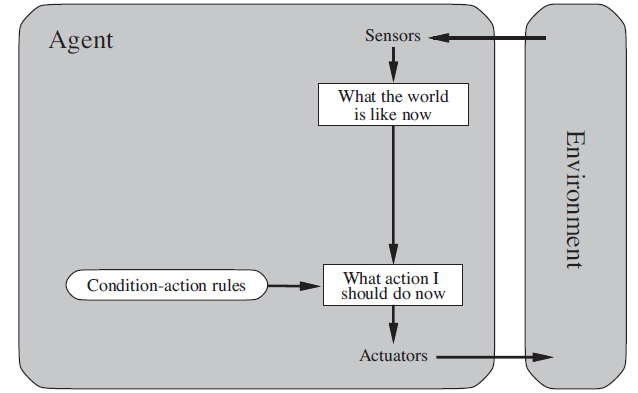
\includegraphics[scale=0.6]{ml1.png}
            \caption{Simple Reflex Agent}
            \label{fig:my_label}
        \end{figure}
        \end{enumerate}
        \begin{algorithm}[h]
            \caption{Simple Reflex Agent}
            \begin{algorithmic}[1]
            \Procedure{simple\_reflex\_agent}{\textit{percept}}
            
            \State \textbf{Persistent:} \\
            \State  \textit{rules}: A set of condition-action rules\\
            
            \State $state \gets interpret\_input(percept)$
            \State $rule \gets rule\_match(state, rules)$
            \State $action \gets rule.Action$
            \State \textbf{return} action
            \EndProcedure
            
        \end{algorithmic}
        \end{algorithm}

        \item \textbf{Model-based agents:}
        
        \begin{enumerate}
            \item To solve the problem of partial observability, model-based agents use the knowledge from past percepts encoded in the form of an internal \textit{model}.
            
            
            \item The model is the agent's means of knowing how a given action will affect the envt, based on a past history of actions and their effects taken by the agent. 
            
        \end{enumerate}
        
        \begin{figure}[ht]
            \centering
            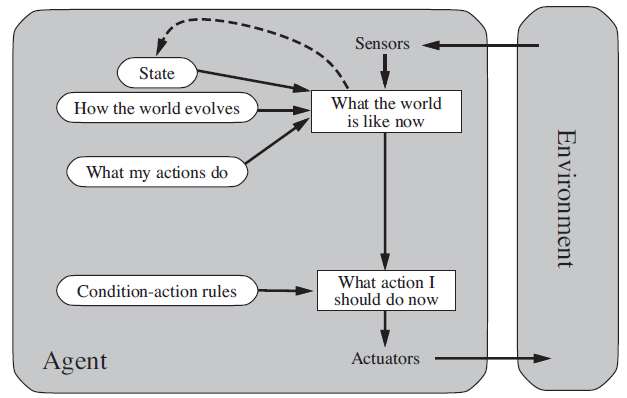
\includegraphics[scale=0.6]{ml2.png}
            \caption{Model Based Agent}
            \label{fig:my_label_2}
        \end{figure}
        
        \begin{algorithm}[ht]
            \caption{Model Based Agent}
            \begin{algorithmic}[1]
            \Procedure{model\_based\_agent}{\textit{percept}}
            \State \textbf{Persistent:} 
            \State \textit{state}: Current world state
            \State \textit{model}: description of how next state depends on current state + action
            \State  \textit{rules}: A set of condition-action rules
            \State \textit{actions}: The most recent action \\
            
            
            \State $state \gets update\_state(state, action, percept, model)$
            \State $rule \gets rule\_match(state, rules)$
            \State $action \gets rule.Action$
            \State \textbf{return} action
            \EndProcedure
            
            \end{algorithmic}
        \end{algorithm}
        \break
        \item \textbf{Goal-based Agents:}
        \begin{enumerate}
            \item Goal-based agents further expand on the capabilities of the model-based agents, by using “goal” information.
            
            \item The goal describes the favourable or most desired outcome of the action taken by an agent. The goal-based agent will take this goal into account as well as the result of the model's computation while deciding the next action.
            
            \item It is possible to define a measure of how desirable a particular state is (instead of a Boolean notion of desirable vs not desirable). This measure can be obtained through the use of utility function which maps a state to measure of the utility of the state (such an agent is called an \textbf{utility-based} agent. 
            
            \begin{figure}[h]
                \centering
                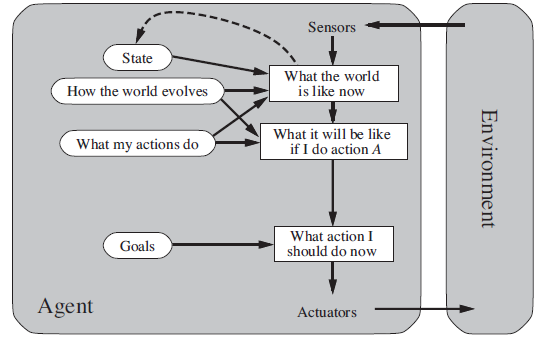
\includegraphics{ml3.png}
                \caption{A model-based goal-based agent}
                \label{fig:my_label_3}
            \end{figure}
        \end{enumerate}
        
        \item \textbf{Learning Agents:}
        \begin{enumerate}
            \item Learning has an advantage that it allows the agents to initially operate in unknown environments and to become more competent that its initial knowledge alone might allow
            
            \item The two elements of a learning model are the \textbf{learning element} which is responsible for making improvements and the \textbf{performance element} which is responsible for selecting external actions.
            
            \item The learning element uses feedback from the critic on how the agent is doing and determines how the performance element should be modified to do better in the future
            
            \item The last component of the learning agent is the \textbf{problem generator}.It is responsible for suggesting actions that will lead to new and informative experiences.
            
            \begin{figure}[ht]
                \centering
                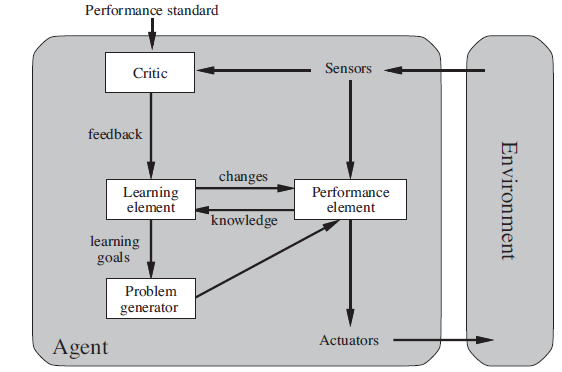
\includegraphics{ml4.png}
                \caption{Learning Agent}
                \label{fig:my_label_4}
            \end{figure}

        \end{enumerate}
    \end{enumerate}
    
     
    
    \subsection{Sensors}
    
    Sensors are devices that capture a proper subset of all the observable variables in the environment at a single point in time. \\
    The information on the current state of the environment that is captured by the sensor is called a \textbf{percept}.\\
    The agent's next course of action is determined either by the current percept or a sequence of past percepts.\\
    An agent can resort to \textbf{probing}, ie. taking some actions to modify the future percepts so that useful information may be obtained. 
    
    \subsection{Environment}
    \begin{defn}
    The environment is a proper subset of the surroundings of an agent that is of interest to that agent, and is important for the agent to achieve its goal.
    \end{defn}
    
    \subsubsection{Properties of an environment:}
    
    \begin{enumerate}
        \item \textbf{Observability:}
        \begin{enumerate}
            \item Fully Observable: All the variables in the environment can be fully captured at any given point in time
            
            \item Partially Observable: Only some variables in the environment can be captured at any given point in time (eg: playing a game of cards, the agent does not know for sure which card will be drawn next from the deck)
        \end{enumerate}
        \item \textbf{Determinism:}
        \begin{enumerate}
            \item Deterministic: The next state of the environment can be fully described based on its current state and the actions taken by the agent.
            
            \item Stochastic: The next state of the environment is not completely determined, ie. there is an element of randomness in the choice of next state.\\
            The word stochastic is used and not non-deterministic as there is a probability attached to the future outcomes of the action taken.\\
            NOTE: partially observable elements \textit{appear} to be stochastic in nature.
        \end{enumerate}
        \item \textbf{Episodicity:}
        \begin{enumerate}
            \item Episodic: The agent's experience is divided into discrete episodes. In each episode the agent receives a percept and takes a single action. The next episode does not depend on any actions taken in any previous episodes. (eg: classification tasks)
            
            \item Sequential: The behaviour of future episodes depends on the action taken in the current episode
        \end{enumerate}
        \item \textbf{Dynamism:}
        \begin{enumerate}
            \item Static: The environment changes only because of an action taken by the agent. No changes may take place while the agent is deliberating (ie. thinking about) its next action.
            
            \item Dynamic: The environment changes even when no action is taken by the agent. A dynamic envt continuously asks the agent about it's next course of action, and if the agent has not finished thinking about it yet then it counts as no action taken.
        \end{enumerate}
        \item \textbf{Continuity:}
        \begin{enumerate}
            \item Discrete: The envt has a discrete number of states, a discrete number of possible percepts and a discrete number of possible actions taken by the agent. (eg: a game of chess)
            \item Continuous: The envt has a continuously varying number of states, possible percepts and future actions possible. (eg: taxi driving)
        \end{enumerate}
    \end{enumerate}
    
\section{Search Strategies in Machine Learning}
Searching is one possible problem solving technique as it allows an agent with several
immediate options of unknown value to decide what to do by first examining future actions that eventually lead to states of known value.

\subsection{Problem Definition}
Any search problem can be defined as per the following criteria:
\begin{itemize}
    \item The \textbf{initial state} of the agent
    
    \item A description of all possible actions of the agent, given the current state. For example, $ACTION(s)$ returns a set of all possible actions from the current state $s$. 
    
    \item A description of all possible results, or a \textbf{transition function}. The function $RESULT(s, a)$ returns the result state of taking action $a$ while being at state $s$. 
    
    \item The transition function, the initial state and the actions form the \textbf{state space} which can be represented as a directed graph, where each node is a result state and each edge is an action to be taken.
    
    \item The \textbf{goal state} determines the point at which the problem is said to have been solved. 
    
    \item The \textbf{path cost} function which assigns a cost to each action (ie. each edge of the graph). 
\end{itemize}

In any graph search algorithm, the \textbf{frontier} is defined as the list of nodes which are yet to be explored. 

There are two main types of search algorithms, \textbf{uninformed} and \textbf{informed}.

\subsection{Uninformed Search Algorithms}

They are called uninformed as they do not know whether a particular state is closer to the goal state or not. All they can do is check if it a state is a goal state or not and then expand each state if it is not a goal state. 

\subsubsection{Breadth First Search (BFS)}

\begin{itemize}
    \item The \textit{shallowest unexpanded node} is always explored first. 
    
    \item This is achieved by using a \textbf{FIFO queue} as the frontier. 
    
    \item Thus, new nodes (which are always deeper than their parents) go to the back of the queue, and old nodes, which are shallower than the new nodes, get expanded first.
    
    \begin{figure}[ht]
        \centering
        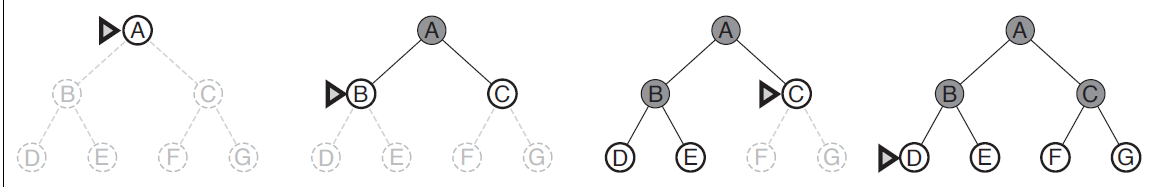
\includegraphics[scale=0.65]{ml5.png}
        \caption{Breadth First Search}
        \label{fig:my_label_5}
    \end{figure}
\end{itemize}
The pseudocode for a BFS algorithm is described below. 
\begin{algorithm}
    \caption{Breadth First Search}
    \begin{algorithmic}
        \Procedure{breadth\_first\_search}{\textit{problem}}
            \State $ node \gets $ a node with STATE=\textit{problem}.INITIAL\_STATE, PATH\_COST=0
            \If {node.STATE == \textit{problem}.GOAL\_STATE}
                \State return SOLUTION(\textit{node})
            \EndIf
            
            \State \textit{frontier} $\gets$ FIFO queue with node as the only element.
            \State \textit{explored} $\gets$ Empty set
            
            \While{frontier \textbf{is not} empty}
                \State \textit{node} $\gets$ POP(\textit{frontier})
                \State add \textit{node}.STATE to \textit{explored}

                \For {action in \textit{problem}.ACTIONS(\textit{node}.STATE)}
                    \State $ child \gets$ CHILD\_NODE(\textit{problem, node, action})
                    \If{\textit{child}.STATE \textbf{not in} \textit{explored}, \textit{frontier}}
                        \If{\textit{child}.STATE == \textit{problem}.GOAL\_STATE}
                            \State return SOLUTION(child)
                            \
                        \EndIf
                        \State \textit{frontier}.insert(child)
                    \EndIf
                \EndFor
            \EndWhile
        \EndProcedure
    \end{algorithmic}
\end{algorithm}

\subsubsection{Uniform Cost Search}
\begin{itemize}
    \item Instead of expanding the shallowest unexpanded node, the uniform-cost search algorithm explores the node with the \textit{lowest path cost}. 
    
    \item Instead of a FIFO queue, the frontier of unexplored nodes is stored as a \textbf{priority queue} stored in order of the path cost. 
    
    \item The goal test is applied on the node only when it is selected for expansion, and not as soon as it is generated. 
    
    \item The pseudocode for the UCS algorithm is described below.

\end{itemize}
\break

\begin{algorithm}
    \caption{Uniform Cost Search}
    \begin{algorithmic}
        \Procedure{Uniform\_Cost\_Search}{problem}
            \State $node \gets $ a node with STATE=\textit{problem}.INITIAL\_STATE, PATH\_COST = 0
            
            \State $frontier \gets $ a priority queue ordered by PATH\_COST, with \textit{node} as the only element
            
            \State $explored \gets$ an empty set
            
            \While{frontier \textbf{is not} empty}
                \State $node \gets $ POP(\textit{frontier})
                \If{node.STATE == problem.GOAL\_STATE}
                    \State \textbf{return} \textit{node}
                \EndIf
                \State add \textit{node}.STATE to \textit{explored}
                \For{action in PROBLEM.actions(node.STATE)}
                    \State $child \gets$ CHILD\_NODE(\textit{problem}, \textit{node}, \textit{action})
                    
                    \If{\textit{child.STATE is not in \textit{explored, frontier}}}
                        \State $frontier \gets$ INSERT(\textit{child, frontier})
                    \ElsIf{\textit{child}.STATE is in \textit{frontier} with higher PATH\_COST}
                        \State replace that \textit{frontier} node with \textit{child}
                    \EndIf
                \EndFor
            \EndWhile
        \EndProcedure
    \end{algorithmic}
\end{algorithm}


\subsubsection{Depth First Search}
\begin{itemize}
    \item Depth-first search always expands depth first \textit{the deepest node} in the current frontier of the search tree.
    
    \item The search proceeds immediately to the deepest level of the search tree, where the nodes have no successors. As those nodes are expanded, they are dropped from the frontier, so then the search \textit{recursively backtracks} to the next deepest node that still has unexplored successors.
    
    \item The frontier is implemented as a linear LIFO data structure called a \textbf{stack}.
    
    \item Without having a check for whether a node has already been visited once, the Depth First Search algorithm is \textit{incomplete} 
\end{itemize}

\begin{algorithm}
    \caption{Depth First Search}
    \begin{algorithmic}
        \Procedure{depth\_First\_search}{problem}
            \State $root\_node \gets $ Make\_Node(problem.INITIAL\_STATE)
            \State $DFS(problem, root\_node)$
        \EndProcedure\\
        
        \Procedure{DFS}{problem, root\_node}
            \If{\textit{root\_node}.STATE == \textit{problem}.GOAL\_STATE}
                \State \textbf{return} SOLUTION(\textit{node})
            \Else 
                \State \textbf{return} failure
            \EndIf
            \For{action in \textit{problem}.ACTIONS(\textit{node}.STATE)}
                \State $child \gets$ CHILD\_NODE(\textit{problem, node, action})
                \State $result \gets$ DFS(problem, child)
            \EndFor
        
        \EndProcedure
    \end{algorithmic}
\end{algorithm}
\subsection{Informed Search Algorithms}
\begin{itemize}
    \item Such algorithms are said to be informed as they contain within them a \textbf{heuristic} that offers an informed guess of the distance from the current node's state to the goal state of the problem. 
    
    \item The \textit{heuristic function} $h(n)$ takes a node $n$ as input and estimates the shortest distance (ie. the length of the path with the least cost) from the state of that node $n$ to the node whose state is the goal state of the problem.  
    
    \item In an Informed search algorithm, the order in which nodes in the frontier are to be explored is decided by the \textit{evaluation function} of a node, $f(n)$. The node having the lowest evaluation value is expanded first by the algorithm. 
\end{itemize}

\subsubsection{Greedy Best-First Search}
\begin{itemize}
    \item The evaluation function in this case is simply the estimate of the cost from the current node state to the goal, ie. the heuristic itself. In other words, $f(n) = h(n)$
    
    \item The frontier is a priority queue ordered by the value of $f(n)$, the evaluation function. 
\end{itemize}

\subsubsection{A* Search}
\begin{itemize}
    \item The evaluation function $f(n)$ in this case is the total estimated cost of the solution starting from the initial state to the goal state. 
    
    \item This incorporates the cost of the path already travelled to the node $n$, given by the function $g(n)$ and the heuristic function's ($h(n)$) guess of the distance to the goal state. 
    
    \begin{equation}
        f(n) = h(n) + g(n)
    \end{equation}
    
    \item Just as in Greedy Best-First Search, the frontier is a priority queue ordered by the value of $f(n)$. 
\end{itemize}

\subsubsection{Characteristics of Heuristic Functions}
Heuristic functions must have the following behaviours:
\begin{itemize}
    \item \textbf{Admissibility:} 
    \begin{enumerate}
        \item For a heuristic function to be admissible, it must never \textit{overestimate} the actual cost to reach the goal state from the current state.
        
        \item Admissible heuristics are by nature optimistic because they think the cost of solving the problem is less than it actually is.
    \end{enumerate} 
    
    \item \textbf{Consistency/Monotonicity}
    \begin{enumerate}
        \item A heuristic $h(n)$ is consistent if, for every node $n$ and every successor $n^\prime$ of $n$ generated by an action $a$, the estimated cost of reaching the goal from $n$ is no greater than the step cost of getting to $n^\prime$ plus the estimated cost of reaching the goal from $n^\prime$.
        
        \begin{equation}
            h(n) \leq cost(a, n, n^\prime) + h(n^\prime)
        \end{equation}
        
        Where $cost(a, n, n^\prime)$ is the cost of the transition caused by action $a$ from node $n$ to its child $n^\prime$.
        
        \item Consistency implies admissibility and this can be easily proven. 
    \end{enumerate}
\end{itemize}

\section{Characteristics of Search Algorithms}

\begin{itemize}
    \item \textbf{Completeness:} The algorithm is guaranteed to find a solution if one exists
    
    \item \textbf{Optimality:} The algorithm finds the \textit{optimal} solution (ie. the one with the least cost). 
    
    \item \textbf{Time Complexity:} Time needed to find a solution.
    
    \item \textbf{Space Complexity:} Space (storage) needed to find a solution.
\end{itemize}

\begin{table}[ht]
    \centering
    \begin{tabular}{|c|c|c|c|c|}
        \hline
        \textbf{Algorithm} & \textbf{Complete} & \textbf{Optimal} & \textbf{Time Complexity} & \textbf{Space Complexity}\\
        
        \hline 
        
        \textbf{Breadth-First Search} & Yes & Yes & $O(b^d)$ & $O(b^d)$ \\
        
        \hline
        
        \textbf{Depth-First Search} & No & No & $O(b^d)$ & $O(bd)$ \\
        
        \hline 
        
        \textbf{Uniform Cost Search} & Yes & Yes & $O(b^{1 + C^*/ \epsilon})$ & $O(b^{1 + C^*/ \epsilon})$ \\
        
        \hline 
    \end{tabular}
    \caption{Comparision of Search Strategies}
    \label{tab:my_label_xxx}
\end{table}

\section{Concept Learning}
\begin{itemize}
    \item A \textbf{concept} is a fact or a generalization about the real world that an agent is supposed to learn given some data that is relevant to that fact.
    
    \item Concept Learning is the act of inferring a Boolean-valued function from the given training examples (eg: inferring whether I will play tennis or not based on the overhead conditions, humidity, temperature and whether it is raining or not).
    
    \item The \textbf{hypothesis} is that function of the inputs which best generalizes the outcomes, as learnt from the training data. 
    
    \item In a concept learning situation, the hypothesis is represented as an $n$-tuple where $n$ is the number of input variables. 
    
    \item The most general hypothesis is denoted as ?, which means any value of that variable will contribute to the correct hypothesis. 
    
    \item The least general hypothesis (ie. the most specific) is denoted as $\phi$, which means that no value of that variable will contribute to the valid hypothesis.
    
    \item Given $n$ features where feature $f_i$ can take $k_i$ values, the number of total features learnt is $k_1 \times k_2 \times ... \times k_n$, number of \textbf{syntactically different concepts} is $(k_1+2) \times (k_2 + 2) \times ... \times (k_n+2)$ and number of \textbf{semantically different concepts} is $(k_1+1) \times (k_2 + 1) \times ... \times (k_n+1) + 1$. 
    
    \item In the following example, the concept to be learnt is EnjoySport. The input variables are described, and the task is to learn a hypothesis that can generalize the correct value of the EnjoySport concept given some new unseen training example.
\end{itemize}
\begin{table}[ht]
    \centering
    \begin{tabular}{|c|c|c|c|c|c|c|}
    \hline
        \textbf{Sky} & \textbf{AirTemp} & \textbf{Humidity} & \textbf{Wind} & \textbf{Water} & \textbf{Forecast} & \textbf{EnjoySport} \\
    \hline
        Sunny & Warm & Normal & Strong & Warm & Same & Yes\\
    \hline
        Sunny & Warm & High & Strong & Warm & Same & Yes \\
    \hline
        Rainy & Cold & High & Strong & Warm & Change & No \\
    \hline
        Sunny & Warm & High & Strong & Cool & Change & Yes \\
    \hline
    \end{tabular}
    \caption{Example for concept learning, target concept: EnjoySport}
    \label{tab:my_label}
\end{table}

\begin{itemize}
    \item The most general hypothesis is represented as $(?, ?, ?, ?, ?, ?)$, ie. any day is a positive example. The most specific hypothesis is represented as $(\phi, \phi, \phi, \phi, \phi, \phi)$ ie. no day is a positive example. 
    
    \item The learner is presented an example of the form $\langle x, c(x) \rangle$ where $x \in X$ is a single training example from the set $X$ of all training examples, and $c(x)$ is the target concept corresponding to  example $x$. Examples for whihc $c(x) = 1$ are called \textit{positive examples} while examples for which $c(x) = 0$ are called negative examples
    
    \item The hypothesis $h: X \rightarrow \{0, 1\}$ is a function that satisfies the constraint $h(x) = c(x) \forall x \in X$
    
    \item The fundamental assumption behind all such hypotheses is that they can only generalize a given training set of examples. Hence, any function that can generalize the target concept well over a \textit{large} set of training examples will also generalize the target concept well on a set of unseen examples.
    
    \item This assumption is called the \textbf{inductive learning hypothesis}.
\end{itemize}

\subsection{Find-S Algorithm}
\begin{itemize}
    \item The Find-S algorithm is used to get the best hypothesis $h$ given a set $X$ of training examples and a concept $c(x)$ to be learnt. 
\end{itemize}

\begin{algorithm}[H]
        \caption{Find-S Algorithm}
        \begin{algorithmic}
        \Procedure{Find\_S}{X}
            \State $h \gets (\phi, \phi, \phi, ..., \phi)$
            \For{$\langle x,c(x) \rangle$ in $X, c$}
                \If{c(x) == 1}  \Comment{x is a positive example}
                    \For{$a_i$ in $h$}
                        \State $a_i \gets a_i \oplus x$
                    \EndFor
                \EndIf
            \EndFor
            \State return $h$
        \EndProcedure
    \end{algorithmic}
\end{algorithm}

\begin{itemize}
    
    \item The $\oplus$ operator denotes the pairwise AND operation, defined as
    \[ a_h \oplus a_x = 
    \begin{cases}
     a_x \text{ if } a_h = \phi \text{ or } a_h = a_x\\
     
     ? \text{ if } a_h \neq a_x \text{ or } a_h = ?
     
    \end{cases}
    \]
    \item Given the examples in table 2, the initial hypothesis being $(\phi, \phi, \phi, \phi, \phi, \phi)$.
    
    \item After the first example, the hypothesis becomes (sunny, warm, normal, strong, warm, same)
    
    \item After the second example, the hypothesis becomes (sunny, warm, ?, strong, warm, same)
    
    \item The third example is ignored as it is a negative example.
    
    \item After the fourth example, the hypothesis becomes (sunny, warm, ?, strong, ?, ?), which is the final hypothesis.
\end{itemize}

\subsubsection{Drawbacks of Find-S}
\begin{itemize}
    \item Find-S has no guarantees that it will output the \textit{only} correct hypothesis, it can output one out of all the correct ones. In other words, it can't give information about the \textit{convergence} of the learning process to a single solution.
    
    \item There is no inherent reason for prefering the most specific possible hypothesis that Find-S outputs. 
    
    \item Find-S is highly sensitive to noise and errors in the training data, as it ignores all negative examples entirely. 
\end{itemize}

\section{Decision Tree Learning}
\begin{itemize}
    \item Decision Tree is a method to approximate a \textbf{discrete-valued} target function, where the learned function is represented as a tree. 
    
    \item Decision Trees are very easy to understand for human beings, as they can be easily coded into a set of \textit{if-else} rules, ie. a \textbf{disjunction of conjunctions}.
    
    \item Decision Trees are classified as \textbf{eager learners} as they try to generalize the training data while being trained on it, in constrast to lazy learners that generalize the training data only when a query is made to them (while testing). 
\end{itemize}

\subsection{Appropriate Problems for DT Learning}
\begin{itemize}
    \item Instances are represented as attribute-value pairs
    
    \item The target function has discrete output values (DTs can be extended to approximate real-valued target functions even though this is rare)
    
    \item Data may contain errors or missing values. DTs are robust to both these defects in the data.
\end{itemize}

\subsection{ID3 Algorithm for Decision Tree Construction}
\begin{itemize}
    \item The ID3 algorithm splits the attribute set at each level based on the \textbf{information gain} from each attribute at each level. 
    
    \item The information gain calculation relies on the calculation of the \textbf{entropy} of the attribute, which is a measure of the impurity (ie. heterogeneity) within a particular sample.
    
    \begin{defn}
    The entropy of a set of examples $S$ defines the number of bits that are needed to encode the classification of any arbitrary member of the set.
    \end{defn}
    
    \item The entropy of a set of examples $S$ having $c$ possible output classes is calculated using the formula
    
    \begin{equation}
        Entropy(S) = - \sum_{i=1}^{c} \frac{n_i}{N} log_{2} \frac{n_i}{N}
    \end{equation}
    
    Where $n_i$ is the number of examples in class $i$ and $N$ is the total number of examples.
    
    \item The \textbf{average entropy} of an attribute $A$ that can take $c$ values is defined as:
    
    \begin{equation}
            E_{avg}(A) = \sum_{i=1}^{c} \frac{p_i}{N} Entropy(i)
    \end{equation}
    
    \item The information gain of attribute $A$ with respect to the dataset of examples $S$ is then defined as
    
    \begin{equation}
        Gain(S, A) = Entropy(S) - E_{avg}(S_i)
    \end{equation}
    
    \item $S_i$ is the subset of $S$ where the attribute $A$ takes the value i. 
\end{itemize}

\subsubsection{Example for Information Gain Calculation}
\begin{itemize}
    \item Suppose the dataset $S$ has 14 examples, and one of the attributes is \textit{wind}.
    
    \item The \textit{wind} attribute can take 2 values, \textit{strong} (8 examples out of 14) and \textit{weak} (6 examples out of 14). 
    
    \item Out of 8 examples where \textit{wind} is \textit{strong}, 6 are positive and 2 are negative
    
    \item Out of 6 examples where \textit{wind} is \textit{weak}, 3 are positive and 3 are negative
    
    \item In the dataset $S$ there are 9 positive and 5 negative examples out of 14.
    
    \item The entropy of the dataset $S$ is given as
    
    \begin{equation*}
        Entropy(S) = - \frac{9}{14} log_{2} \frac{9}{14} - \frac{5}{14} log_{2} \frac{5}{14} = 0.9402
    \end{equation*}
    
    \item The Entropy values for the \textit{strong} and \textit{weak} classes of attribute \textit{wind} are
    
    \begin{equation*}
        Entropy(S_{strong}) = -\frac{2}{8} log_{2} \frac{2}{8} - \frac{6}{8} log_{2} \frac{6}{8} = 0.811
    \end{equation*}
    
    \begin{equation*}
        Entropy(S_{weak}) = -\frac{3}{6} log_{2} \frac{3}{6} - \frac{3}{6} log_{2} \frac{3}{6} = 1
    \end{equation*}
    
    \item Then the Information gain of attribute \textit{wind} can be calculated as
\end{itemize}
\begin{align*}
        Gain(S, wind) &= Entropy(S) - \left[\frac{8}{14} Entropy(S_{strong}) + \frac{6}{14} Entropy(S_{weak})\right] \\
        &= 0.9402 - \left[\frac{8}{14} 0.811 + \frac{6}{14} 1\right] \\
        &= 0.048
\end{align*}

\begin{itemize}
    \item The ID3 algorithm recursively splits the data set $S$ based on the attribute which has the highest information gain, until no more splitting can be done. 
    
    \item The ID3 algorithm is a \textit{greedy algorithm} that takes the best possible choice at the current state of the problem. 
\end{itemize}

\subsection{The Inductive Bias of the ID3 Algorithm}
\begin{itemize}
    \item The bias of the ID3 algorithm can be characterized by the way it keeps attributes with the highest information gain at the top. This implies a preference for short and fat decision trees over tall and thin trees.
    
    \item \textbf{Bias:} The ID3 algorithm prefers shorter trees, and prefers trees which have attributes with large information gain closer to the root. 
    
    \item This is an argument derived from \textbf{Occam's Razor} which is an inductive hypothesis that states that the simplest hypothesis that fits the data must be selected. 
\end{itemize}

\section{Issues in Decision Tree Learning}
\subsection{Overfitting}
\begin{defn}
    Given a hypothesis space $H$, a hypothesis $h \in H$ is said to \textbf{overfit} the training data if there exists an alternate hypothesis $h' \in H$ such that $h$ has a smaller error than $h'$ over the training data but $h'$ has a smaller error than $h$ over the entire set of examples. 
\end{defn}

\begin{itemize}
    \item Overfitting essentially means that the hypothesis is the result of the model \textbf{memorizing} the training data that was input into it, instead of generalizing the data properly.
    
    \item Approaches that prevent overfitting in Decision Trees can be grouped into two:
    \begin{itemize}
        \item \textbf{Pre-Pruning Approaches}: Those that stop growing the tree \textit{before} it reaches the point where the training data is perfectly classified.
        
        \item The growth is stopped when the goodness of the split falls below a certain threshold. The goodness can be measured using the information gain.
        
        \item The value of the threshold, however, is hard to estimate well for different situations.
        
        \item \textbf{Post-Pruning Approaches}: Those that allow the tree to grow to its full extent and overfit the data, and then prune the tree
    \end{itemize} 
    
    \item The final correct size of the tree may be evaluated by
    \begin{itemize}
        \item Use a separate validation data set to find the utility (ie. usefulness) of post pruning
        
        \item Use of statistical tests to determine whether expanding a particular node is likely to produce an improvement over the entire data set. (eg: $\chi^2$ test)
        
        \item Use of an explicit measure of complexity in encoding the training examples and the decision tree, and halting the growth when this complexity is minimized. 
    \end{itemize}
\end{itemize}

\subsubsection{Reduced Error Pruning}
\begin{itemize}
    \item The process of pruning a tree consists of removing the subtree attached to that node (making it a leaf node), and then assigning the most common classification of examples attached to that node to the new leaf node. 
    
    \item In reduced error pruning, a pruning operation is done only if the resultant tree offers equivalent or better performance over the validation set. 
    
    \item Pruning is done iteratively until further pruning will result in a drop in performance over the validation set. 
    
    \item The drawback of this approach is that since it requires a validation set of examples to evaluate the pruning, it is not suitable for situations where limited amount of data is available. 
\end{itemize}

\subsubsection{Rule Based Post Pruning}
\begin{itemize}
    \item This algorithm follows the following procedure:
    \begin{itemize}
        \item Grow the decision tree to the largest possible extent and allow it to overfit the train data.
        
        \item Convert the learned tree into a set of rules by building one rule for each path from root to all leaf nodes.
        
        \item Prune each rule by removing any preconditions that result in improvement in estimated accuracy. No pruning is done if it results in a drop in estimated accuracy
        
        \item Sort the pruned rules by their estimated accuracy, and consider them in this sequence when classifying subsequent instances
    \end{itemize}
    
    \item The tree-to-rule conversion is done \textit{before} the pruning for the following reasons.
    \begin{itemize}
        \item It allows pruning to happen on the basis of a particular context instead of taking one broad decision that affects the entire decision tree (ie. removing or retaining one entire node).
        
        \item Any distinction between root and leaf nodes with respect to testing is removed, hence the structure of the tree becomes easier to maintain (as against the tree pruning where the root may be pruned but the subtrees are intact).
        
        \item Improves readability for humans
    \end{itemize}
\end{itemize}

\subsection{Dealing with Continuous Values}
\begin{itemize}
    \item The ID3 algorithm as presented above is valid only for attributes that take on discrete values.
    
    \item When continuous values are involved, they are converted into discrete attributes by binning.
    
    \item If the attribute $A$ takes on a continous set of values, it can be converted into an attribute $A_c$ by selecting a threshold $c$ such that $A_c$ is true for all examples where $A < c$ and false otherwise. 
    
    \item The value $c$ is chosen at a boundary between the examples that produces the largest information gain value.
    
    \item It can be shown that the value of $c$ that produces the largest information gain lies at a boundary where the current example is positive and the next example is negative or vice versa. 
\end{itemize}

\subsection{Dealing with missing values}
\begin{itemize}
    \item If an example does not have a value for some attribute $A$ which is to be used to split the data at a particular node, then that value can be replaced with the value of $A$ that is most common for all the examples at that node.
    
    \item An alternate approach is to replace with the value of $A$ that is most common among examples at that node which have the same target value $c(x)$
    
    \item A more complex approach is to assign probabilities to each possible value of $A$ and then split the example in the ratio of those probabilities along the possible branches.
\end{itemize}

\section{Performance Metrics}
These are used to evaluate the performance of a trained model, and as goals to determine the ideal model state. 

\subsection{Confusion Matrix}
\begin{itemize}
    \item It is a matrix that lays out the model performance in terms of the actual labels in the data and the predicted labels that were generated by the model. 
    
    \item It is a matrix of the true positives (predicted True, actual label True), false positives (predicted False, actual label True), true negatives (predicted False, actual label False) and false negatives (predicted True, actual label False).
    
    \item Note: The positive/negative in the term refers to whether the \textbf{predicted label} was positive or negative. The True/False in those terms refers to whether prediction and actual label are \textbf{same} or not
\end{itemize}
\begin{figure}[!h]
\centering
    \begin{tabular}{|c|c|c|}
        \hline
        & Predicted True & Predicted False \\
        \hline
        Actual True & TP & FN \\
        \hline
        Actual False & FP & TN \\
        \hline
    \end{tabular}
\end{figure}

\begin{itemize}
    \item Whether minimization of FP is desired or FN is desired is dependent on the use case of the model. 
    
    \item For situations like spam classification, false negatives must be minimized as we don't want a mail that is actually spam (actual label True) to be classified as not spam (predicted label False). 
\end{itemize}

\subsection{Accuracy}
The accuracy of a classifier is given by
\begin{equation}
    Accuracy = \frac{TP + TN}{TP+TN+FP+FN}
\end{equation}

\begin{itemize}
    \item The accuracy is a valid performance measure when the classes occur in the data in balanced  or almost balanced numbers (eg: 50-50 split, 60-40 split)
    
    \item If the dataset is highly skewed to one set, then maximising the accuracy does not mean much. 
    
    \item eg: If the dataset has 97\% data belonging to class $c_1$ and 3\% to class $c_2$, and if a classifier outputs $c_1$ all the time then it still has an accuracy of 97\% despite clearly being a terrible classifier model. 
\end{itemize}

\subsection{Precision}
The precision of the classifier is given by
\begin{equation}
    Precision = \frac{TP}{TP+FP}
\end{equation}
\begin{itemize}
    \item It denotes the fraction of correctly classified \textbf{positive} examples, ie. how many of the selected items are relevant
    
    \item It is used when false positives are significant and must be minimized.
\end{itemize}

\subsection{Recall}
The recall of the classifier is given by
\begin{equation}
    Recall = \frac{TP}{TP+FN}
\end{equation}
\begin{itemize}
    \item It is also referred to as the \textit{sensitivity}
    
    \item It denotes the fraction of incorrectly classified \textbf{positive} examples, ie. how many of the relevant items were selected. 
    
    \item It is used when false negatives are significant and must be minimized.
\end{itemize}
\begin{figure}[!ht]
    \centering
    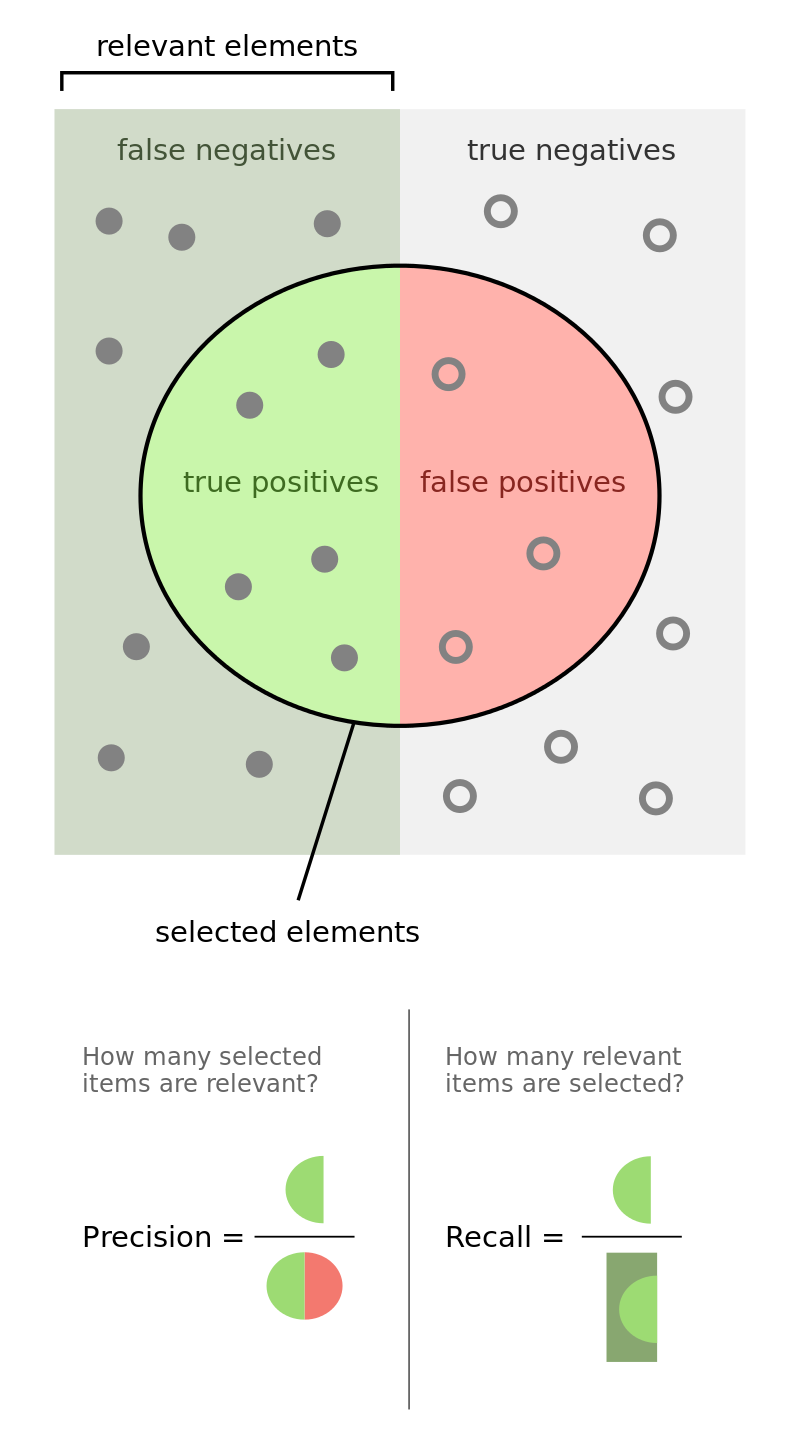
\includegraphics[scale=0.2]{prec_recl.png}
    \caption{Precision and Recall}
    \label{fig:my_label_6}
\end{figure}

\subsection{Specificity}
It denotes the number of correctly classified negative examples. 
\begin{equation}
    Specificity = \frac{TN}{TN+FP}
\end{equation}

\subsection{The $F_1$ Score}
It is the harmonic mean of precision and recall
\begin{equation}
    F_1 = \frac{2 P R}{P + R}
\end{equation}

\subsection{Receiver Operator Characteristics}
\begin{itemize}

    \item The Receiver Operator Characteristics (ROC) is a curve plotted for binary classifiers for various thresholds for classification. 
    \item The x-axis represents the False Positive Rate which is given as $1-Specificity$ (FPR)
    
    \item The y-axis represents the True Positive Rate which is known as $Recall$ (TPR)
    
    \item The area under the ROC curve (also called the AUC) is a measure of the goodness of the classifier (more the area, better the classifier).
    
    \item If AUC=1, then the classifier does a perfect job at classifying on the training set. 
    
    \item If $0.5 < AUC < 1$ then there is a high chance that the classifier will be able to distinguish the positive class values from the negative class values. 
    
    \item If $ AUC < 0.5$ then the classifier is not able to distinguish between positive and negative classes. It outputs random labels for all examples or the same label for all examples. 
\end{itemize}
\end{document}
